\documentclass{emulateapj}
%\documentclass[12pt,preprint]{aastex}
\usepackage{graphicx}
\usepackage{float}
\usepackage{amsmath}
\usepackage{epsfig,floatflt}



\begin{document}

\title{Diffraction and angular resolution}

\author{Daniel Heinesen}

\email{daniel.heinesen@sf-nett.no}

\altaffiltext{1}{Institute of Theoretical Astrophysics, University of
  Oslo, P.O.\ Box 1029 Blindern, N-0315 Oslo, Norway}


%\date{Received - / Accepted -}

\begin{abstract}
  State problem. Briefly describe method and data. Summarize main results.
\end{abstract}
\keywords{cosmic microwave background --- cosmology: observations --- methods: statistical}

\section{Introduction}
\label{sec:introduction}

Discuss background, physical importance and possibly some history of
the problem that is being studied in this paper.


\section{Method}
\label{sec:method}


Describe method. Define data model and likelihood. Outline how the
likelihood was computed (grid or MCMC).

Define the power law model in terms of $Q$ and $n$. 


\subsection{Single Slit Experiment}
In this experiment a laser of unknown wavelength, powered by a 4.5 V battery, was placed on simple platform and aimed at a slit with the width of  $a = 100\mu m$. The resulting diffraction pattern was projected on a wall. The distance from the slit to the wall was measured with a tape measurer. The measurements of the maxima were taken. The distance between the maxima was found by projecting the diffraction pattern on a piece of white paper and marking every maxima from the 10th on the left to the 10th on the right with a pencil, and the using a ruler to measure the distance between the 10th maximum and the center on each side, and the distance between the 10th maximum on each side, thus getting 3 different measurement which could be used to get a more accurate result.\\

\textbf{INSERT PICTURE OF SET UP HERE!}\\

\textbf{Kan settes i teori:}

To find the wavelength we use 

\begin{equation}
\sin \theta_{max} \approx \pm (m+1/2)\frac{\lambda}{a}
\end{equation}\label{eq:slitMax}
\begin{equation}
\sin \theta_{max} \approx \pm m\frac{\lambda}{a}
\end{equation}\label{eq:paperClipMax}
\begin{equation}
\theta_{min} = K\frac{\lambda}{d}
\end{equation}\label{eq:diffLimit}

\subsection{Paper Clip and Anti-Slit}
In this experiment the slit was replaced with a paper clip with an unknown width. The rest of the setup was more or less identical as with the single slit experiment, but the laser was moved further back due to the small pattern resulting from the diffraction. This movement of the laser gave a further uncertainty due to the tape measurer being to short to measure the whole distance. Two measurements were used, with two different uncertainties.

As with the single slit a white paper was placed behind the diffraction pattern, and the maxima were marked with a pencil. The distance between the 35th on the left and the right of the midpoint was measured with a ruler.

With data the width of the paper clip was the measured.

\subsection{Diffraction by a Circular Aperture}
For this experiment a laser of known wave length was shinned into an optic fibre. The fibre was connected to a collimator tube with dampening filter -- so to not destroy the camera. A double lens was placed after the tube, to focus the light. In front of this a microscope objective was placed, which magnified the light 20x. Lastly a monochromatic camera connected to a computer was placed in front of the objective to capture the diffraction pattern.

The lens was measured with a ruler.

\textbf{INSERT IMAGE}

The objective had to be placed in the focal point of the lens, $f = 100$ mm. The focal point was at a known distance. But to ensure that the beam was focused and was hitting the objective, a piece of white paper was placed in front of the objective. The lens was then adjusted until the beam hit the objective. The paper was then moved back and forward to see if the light was most concentrated at the focal point. 

Having a picture of the Airy pattern the number of pixels to the first minimum was simply counted, and knowing the size of each pixel and the distance from the objective and the camera, the angle of the first minimum was calculated. From the angle of the first minimum, a value for $K$ was calculated.

\subsection{Arago spot}
The lens, objective and camera was then removed and replaced by a small circular piece of plastic. The resulting pattern was projected on to the wall.

\subsection{JWST} 
Having found the diffraction limit of a lens, the limit for the James Webb Space Telescope(JWST) can be found from \eqref{eq:diffLimit}. 

\subsection{Uncertainties}
\subsubsection{Single slit}
The distance between the slit and the wall was measured with a tape measurer. Due to the flexible nature of the tape measurer, the distance was not measured in a straight line, giving rise to a small uncertainty. A uncertainty of $\pm 0.5 cm$ was added to the distance.

It was also difficult to ensure that the measurement was done in a horizontal line, normal to the wall. The set up it self also contributed to the uncertainty of the measurements: to get a consistent distance between the minima the laser had to be normal to the wall, and the slit in the center of the laser beam. \\

The measurement of the distance of the extrema of the diffraction pattern was done quite crude, so both the marking of the maxima on the paper and the measuring with the ruler lead to uncertainty. The extension of the maxima was taken to be half that of the distance between two adjacent maxima. The error in measurement was estimated to at most one quarter that of this distance, giving us quite a large uncertainty. The error of the ruler was determined to insignificant compared to that of the marking, so only that uncertainty was kept.

To compensate for all these uncertainties, an uncertainty of $\pm 0.1 cm$ was added to the distance to the 10th maxima.


\subsubsection{Paper clip}
The first measurement was from the wall to the table used for the laser and paper clip. Here the same problem as the measurement for the single slit appears, as the tape measurer bends under its own weight, thus measuring a slightly longer distance. 

A second measurement was from the end of the table to the paper clip. Here the tape measurer was place on the table surface, thus there was no bend in the measurer, giving a more precise measurement. 

Since two measurements were done, an uncertainty arose from the difficulty in starting the second measurement where the first ended. So a small uncertainty was added to the second measurement to compensate for this.

Due to the short distance from the paper clip to the wall, the maxima of the diffraction pattern were close together, making the marking of the maxima quite uncertain. This together with uncertainty in the ruler, a certainty of $\pm 0.2 cm$ was added. 

\subsubsection{Diffraction of a Circular Aperture}
Three measurements was the main sources for uncertainty in this experiment.

The distance between the lens and objective was measured with a ruler. the measurement was taken from the start of the objective to the center of the lens. The uncertainty was estimated to be some $\pm 0.5 cm$.

The width of the lens was also measured with a ruler, but was easier to measure, giving only an uncertainty of $\pm 0.2$.

The Airy Disc was contained in very few pixels in the picture. The point of the first minimum may be in-between two pixels, giving an uncertainty of a whole pixel. The center of the Airy disc may also not be in one single pixel, but since the area of the disc is much larger than the point of the minimum, this does not contribute so much to the total uncertainty.

\section{Results}
\label{sec:results}

\subsection{Measurements}
\subsubsection{Single slit}

\begin{table}[H]
\begin{tabular}{ c c c }
Measurement done & Measured value & Unit\\
\hline
Distance laser to wall & $183 \pm 0.5$ & cm \\
Distance from midpoint to 10th max & $12.25 \pm 0.1$ & cm\\
Distance from 10th max to midpoint & $12.40 \pm 0.1$ & cm\\
Distance from 10th max to 10th max & $24.70 \pm 0.1$ & cm\\
Average distance to 10th max & $12.33 \pm 0.23$ & cm\\
\end{tabular}
\caption{The measurements for the single slit experiment.}
\end{table}\label{tab:dataSingleSlit}

\subsubsection{Paper clip}

\begin{table}[H]
\begin{tabular}{ c c c }
Measurement done & Measured value & Unit\\
\hline
Distance from paper clip to end of table & $102.0 \pm 0.5$ & cm \\
Distance from end of table to wall & $120.5 \pm 0.5$ & cm \\
Distance from 35th max to 35th max & $11.6 \pm 0.2$ & cm\\
\end{tabular}
\caption{The measurements for the paper clip experiments.}
\end{table}\label{tab:dataPaperClip}

\subsubsection{Diffraction of a Circular Aperture}

\begin{table}[H]
\begin{tabular}{ c c c }
Measurement done & Measured value & Unit\\
\hline
Wave length of laser & $635$ & nm \\
Distance from lens to objective & $10 \pm 0.5$ & cm\\
Width of lens & $10.0 \pm 0.2$ & cm\\
Pixels from center to first minimum & $3 \pm 1$ & px\\
Size of pixels & $6$ & $\mu$m/px\\
Magnification & 20x & -\\
Distance from center to first minimum & $\frac{18 \pm 6}{20}$& $\mu$m
\end{tabular}
\caption{The measurements for the circular diffraction.}
\end{table}\label{tab:dataAiry}

\begin{figure}[H]
\centering
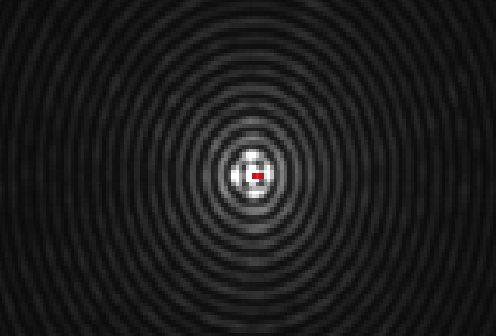
\includegraphics[scale=0.4]{Airy3zoomed2.png}
\caption{Zoomed in picture of the Airy disc. The distance from the center of the disc to the first minimum is marked in red. The distance is 3 pixels.}
\end{figure}

\subsubsection{JWST}
\begin{table}[H]
\centering
\begin{tabular}{ c c c }
Mirror Size & Frequencies \\
\hline
6 m & 600 nm - 28.5 $\mu$m 
\end{tabular}
\caption{Data for the James Webb Space Telescope}
\end{table}\label{tab:dataJWST}

\begin{table}[H]
\centering
\begin{tabular}{ c c c }
Target & Distance $r$ & Smallest Size $r_{min}$ \\
\hline
Near-Earth orbit to Earth & 540 km &$8.1 \pm 2.7$ cm \\
Earth to sun & 1 AU & $22.44 \pm 7.5$ km \\
Solar System to Galactic Center & 8.5 pc & $3.9\cdot 10^7 \pm 1.3\cdot 10^7$ km \\
Milky Way to galaxy formation &  4 billion ly & $184 \pm 61.5$ pc 
\end{tabular}
\caption{The smallest size the JWST can see at different distances. A Skinny triangle approximation is used with the angular resolution found in \eqref{JWSTDiffLimit}.}
\end{table}\label{tab:visionJWST}


\subsection{Calculation}
\subsubsection{Single slit}
The unknown wave length can be calculated as

\begin{equation}
\lambda = \sin \theta_{max}\frac{a}{m+1/2} \approx \theta_{max}\frac{a}{m+1/2}
\end{equation}

From the data in \ref{tab:dataSingleSlit} the angle can be estimated as

\begin{equation}
\theta_{max} \approx \arctan\left( \frac{12.33}{183} \pm 0.0013 \right) = 0.0673 \pm 0.00129
\end{equation}

Which gives 

\begin{equation}
\lambda \approx (0.0673 \pm 0.00129) \cdot \frac{100}{10 +1/2}\text{ }\mu \text{m} 
\end{equation}
\begin{equation}
= 0.641\pm 0.01229\text{ }\mu \text{m} = 641 \pm 12.29 \text{ nm}
\end{equation}\label{eq:waveLenghtLaser}

So based on this experiment, the laser should have a wave length of $641 \pm 12.29 \text{ nm}$.

\subsubsection{Paper Clip}

The width of the paper clip can be found with the use of \eqref{eq:paperClipMin}. The width is given as

\begin{equation}
a \approx \frac{m \lambda}{\theta_{max}}
\end{equation}

The angle can be found as 

\begin{equation}
\theta_{max} \approx \arctan\left(\frac{5.8}{122.5} \pm 0.00086\right) =0.0473 \pm 0.0009
\end{equation}

Giving a a estimated width of

\begin{equation}
a \approx \frac{35\cdot (641 \pm 12.29)}{0.0473 \pm 0.0009} \text{ nm}
\end{equation} 

\begin{equation}
= 0.4743 \pm 0.01281 \text{ mm}
\end{equation}\label{eq:widthPaperClip}

Which gives a width of the paper clip of $0.4743 \pm 0.01281 \text{ mm}$.

\subsubsection{Diffraction of a Circular Aperture}

With the use of \eqref{eq:diffLimit} a value for $K$ can be calculated.

\begin{equation}
K = \frac{\theta_{min} d}{\lambda}
\end{equation}

The angle can be found as

\begin{equation}
\theta_{min} = \arctan\left(\frac{18/20}{100000} \pm 3.005\cdot 10^{-6} \right)
\end{equation}
\begin{equation}
= 9\cdot 10^{-6} \pm 3.005\cdot 10^{-6}
\end{equation}

The value for $K$ can then be calculated as 

\begin{equation}
K = \frac{9\cdot 10^{-6} \pm 3.005\cdot 10^{-6}}{635}\cdot(1\cdot10^8 \pm 2\cdot10^6)
\end{equation}
\begin{equation}
= 1.417 \pm 0.474
\end{equation}\label{eq:K}

So the estimated value is $K = 1.417 \pm 0.474$

\subsubsection{JWST}
From the above results, mainly \eqref{eq:K} we can find the diffraction limit of the James Webb Space Telescope:

\begin{equation}
\theta_{min} = (1.417 \pm 0.474) \cdot \frac{635 \text{ nm}}{6 \text{ m}}
\end{equation}
\begin{equation}
= 1.5\cdot 10^{-7} \pm 5.016\cdot 10^{-8}
\end{equation}\label{JWSTDiffLimit}

This can then be used to find the smallest physical sizes the JWST can see at different distances, with the use of the skinny triangle approximation

\begin{equation}
d_{min} = r\theta_{min}
\end{equation}

These distances can be found in table \ref{tab:visionJWST}
\section{Conclusions}
\label{sec:conclusions}

Summarize results. Discuss their importance, referring to the
discovery to the initial seeds for structure formation. Mention that
these results are in good agreement with expectations from
inflationary theory.



%\begin{figure}[t]
%
%\mbox{\epsfig{figure=filename.eps,width=\linewidth,clip=}}
%
%\caption{Description of figure -- explain all elements, but do not
%draw conclusions here.}
%\label{fig:figure_label}
%\end{figure}


%
%\begin{deluxetable}{lccc}
%%\tablewidth{0pt}
%\tablecaption{\label{tab:results}}
%\tablecomments{Summary of main results.}
%\tablecolumns{4}
%\tablehead{Column 1  & Column 2 & Column 3 & Column 4}
%\startdata
%Item 1 & Item 2 & Item 3 & Item 4
%\enddata
%\end{deluxetable}



\begin{acknowledgements}
  Who do you want to thank for helping out with this project?
\end{acknowledgements}

\begin{thebibliography}{}

\bibitem[G{\'o}rski et al.(1994)]{gorski:1994} G{\'o}rski, K. M.,
  Hinshaw, G., Banday, A. J., Bennett, C. L., Wright, E. L., Kogut,
  A., Smoot, G. F., and Lubin, P.\ 1994, ApJL, 430, 89

\end{thebibliography}


\end{document}